%! TEX root = ../notes/main_notes.tex

\lecture{A Foundational Social Ecological System}{lec-SES2}

\mode<article>{
	Sustainability challenges exist because of the interaction between humans and the environment they inhabit.
	
	Lets consider a system that incorporates humans and the environment.
	
	A simple example is a 'stylized' hunter gatherer model.  In this case, our hunters will harvest fish, building on the model considered earlier.
}

\begin{frame}{The Hunter Gatherer Village}
	\begin{itemize}
		\item The Question: ?
		\begin{itemize}
			\item 1
		\end{itemize}
	\end{itemize}
\end{frame}

\mode<article>{
	An apparently simple mode can become complex pretty quickly.
}

\begin{frame}{The Hunter Gatherer Village}
	\centering
	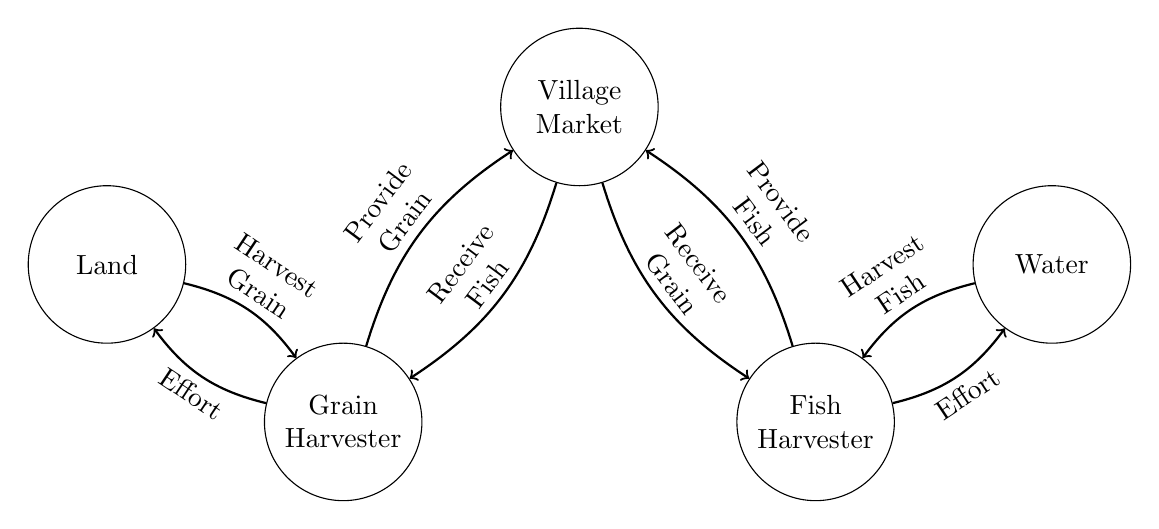
\begin{tikzpicture}
		% Define and place the nodes
		\node [circle, draw, minimum size=2cm, align=center] at (6,6) (village) {Village \\ Market};
		\node [circle, draw, minimum size=2cm, align=center] at (3,2) (gather) {Grain \\ Harvester};
		\node [circle, draw, minimum size=2cm, align=center] at (9,2) (fish) {Fish \\ Harvester};
		\node [circle, draw, minimum size=2cm, align=center] at (0,4) (land) {Land};
		\node [circle, draw, minimum size=2cm, align=center] at (12,4) (water) {Water};
		
		% Draw edges
		\draw [->, thick, align=center] (land) to [bend left=20] node [above, sloped] {Harvest \\ Grain} (gather);
		\draw [->, thick, align=center] (gather) to [bend left=20] node [below, sloped] {Effort} (land);
		\draw [->, thick, align=center] (water) to [bend right=20] node [above, sloped] {Harvest \\ Fish} (fish);
		\draw [->, thick, align=center] (fish) to [bend right=20] node [below, sloped] {Effort} (water);
		\draw [->, thick, align=center] (gather) to [bend left=20] node [above, sloped] {Provide \\ Grain} (village);
		\draw [->, thick, align=center] (village) to [bend left=20] node [above, sloped] {Receive \\ Fish} (gather);
		\draw [->, thick, align=center] (fish) to [bend right=20] node [above, sloped] {Provide \\ Fish} (village);
		\draw [->, thick, align=center] (village) to [bend right=20] node [above, sloped] {Receive \\ Grain} (fish);
	\end{tikzpicture}
\end{frame}

\begin{frame}{The Hunter Gatherer Village}
	\begin{itemize}
		\item The grain subsystem
		\begin{itemize}
			\item Grain grows on the land
			\item Grain harvesters exert effort that translates into harvested grain.
		\end{itemize}
		\item The fish subsystem
		\begin{itemize}
			\item Fish grow in the water
			\item Fish harvesters exert effort that translates into harvested fish.
		\end{itemize}
		\item The Village system
		\begin{itemize}
			\item Fish harvesters bring fish to the village, receive grain.
			\item Grain harvesters bring grain to the village, receive fish.
			\item How is the exchange of fish for grain managed?
		\end{itemize}
	\end{itemize}
\end{frame}

